\documentclass[12pt]{article}
\usepackage[margin=0.2in]{geometry}
\usepackage{amssymb}
\usepackage{amsmath}
\usepackage{url}
\usepackage{bm}
\usepackage{color}
\usepackage{graphicx}
\usepackage{cite}
\usepackage{caption}
\usepackage{subcaption}
\usepackage{hyperref}
\usepackage[section]{placeins} %keeps floats in their own section

\hypersetup{
    colorlinks,
    citecolor=blue,
    filecolor=blue,
    linkcolor=blue,
    urlcolor=blue
}

\newcommand{\red}[1]{{\color{red}{#1}}}
\newcommand{\blue}[1]{{\color{blue}{#1}}}
\newcommand{\ket}[1]{\left| #1 \right>}
\newcommand{\bra}[1]{\left< #1 \right|}
\newcommand{\braket}[2]{\left< #1 | #2 \right>}
\newcommand{\ketbra}[2]{\left| #1 \right> \left< #2 \right|}
\newcommand{\expect}[1]{\left< #1 \right>}
\newcommand{\fpij}{f_p(r_{ij})}
\newcommand{\vpij}{v_p(r_{ij})}
\newcommand{\Opij}{\mathcal{O}_{ij}^p}
\newcommand{\fOpij}{\sum\limits_{i<j}\sum\limits_p \fpij\Opij}
\newcommand{\fqkl}{f_q(r_{kl})}
\newcommand{\Oqkl}{\mathcal{O}_{kl}^q}
\newcommand{\fOqkl}{\sum\limits_{k<l}\sum\limits_q \fqkl\Oqkl}
\newcommand{\fOqklip}{\sum\limits_{k<l,\mathrm{ip}}\sum\limits_q \fqkl\Oqkl}
\newcommand{\fOqklquad}{\sum_{\substack{k<l\\ij \ne kl}}\sum\limits_q \fqkl\Oqkl}
\newcommand{\f}[2]{f_{#1}(r_{#2})}
\renewcommand{\O}[2]{\mathcal{O}_{#2}^{#1}}
\newcommand{\fO}[2]{\sum\limits_{#1} f_{#1}(r_{#2})\mathcal{O}_{#2}^{#1}}
\newcommand{\R}{\mathbf{R}}
\newcommand{\dt}{\Delta\tau}
\newcommand{\ti}{\bm{\tau}_i}
\newcommand{\tj}{\bm{\tau}_j}
\newcommand{\si}{\bm{\sigma}_i}
\newcommand{\sj}{\bm{\sigma}_j}

\title{Plots for Alpha Formation in Mostly Neutron Matter}
\author{Cody L. Petrie}

\begin{document}
\maketitle
\tableofcontents
\newpage

\section{Total Energy Plots for Alpha, 14n, and 14n2p}
\begin{figure}[h!]
   \centering
   \begin{subfigure}{0.49\textwidth}
      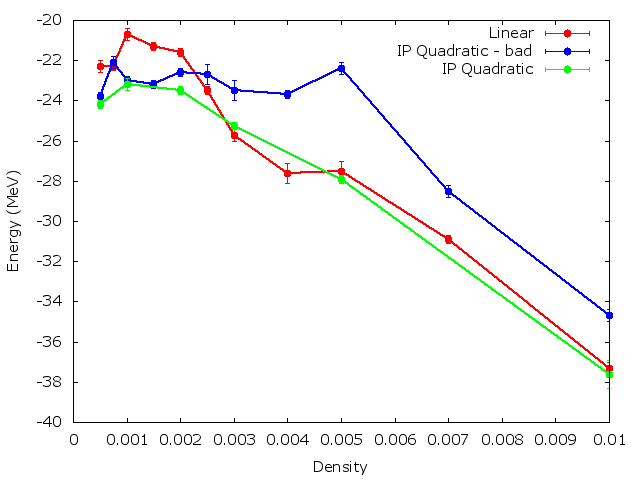
\includegraphics[width=\textwidth]{../alpha.png}
      \caption{Alpha energy calculated as $16\epsilon_{14n2p}-12\epsilon_{14n}$ where $\epsilon=E/A$.}
   \end{subfigure}
   ~
   \begin{subfigure}{0.49\textwidth}
      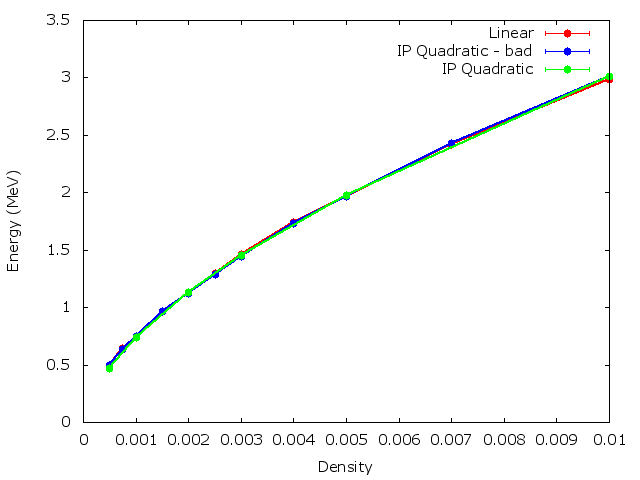
\includegraphics[width=\textwidth]{../14n.png}
      \caption{Energy/particle for 14 neutrons.}
   \end{subfigure}
   ~
   \begin{subfigure}{0.49\textwidth}
      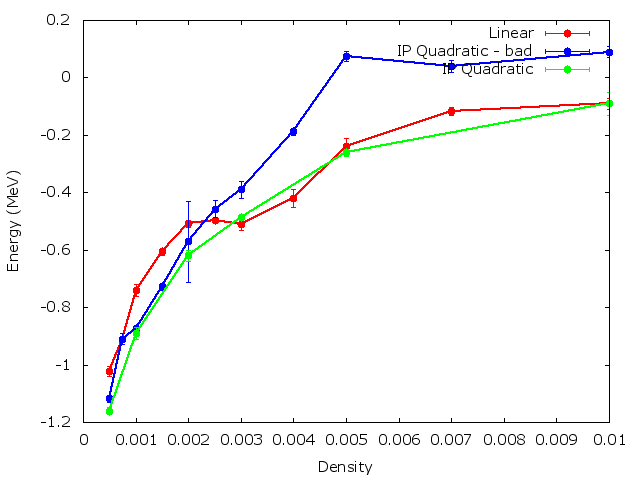
\includegraphics[width=\textwidth]{../14n2p.png}
      \caption{Energy/particle for 14 neutrons + 2 protons.}
   \end{subfigure}
\end{figure}
\newpage

%\section{Energy Plots for Alpha, 14n, and 14n2p - KE}
%\begin{figure}[h!]
%   \centering
%   \begin{subfigure}{0.49\textwidth}
%      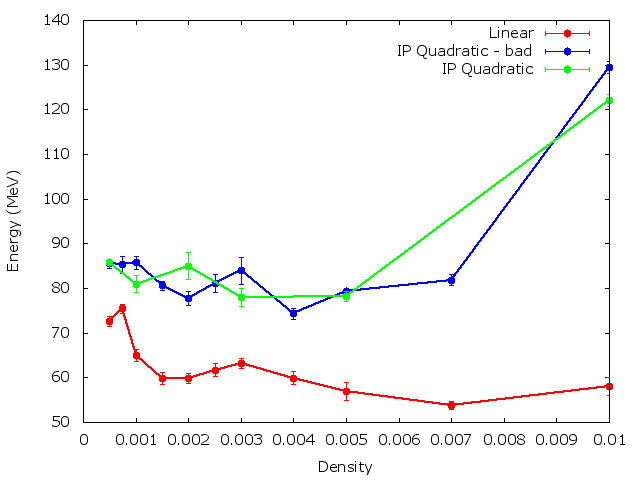
\includegraphics[width=\textwidth]{../alpha_ke.png}
%      \caption{KE of alpha calculated as $16\epsilon_{14n2p}-12\epsilon_{14n}$ where $\epsilon$ are the KE pieces of $\epsilon=E/A$.}
%   \end{subfigure}
%   ~
%   \begin{subfigure}{0.49\textwidth}
%      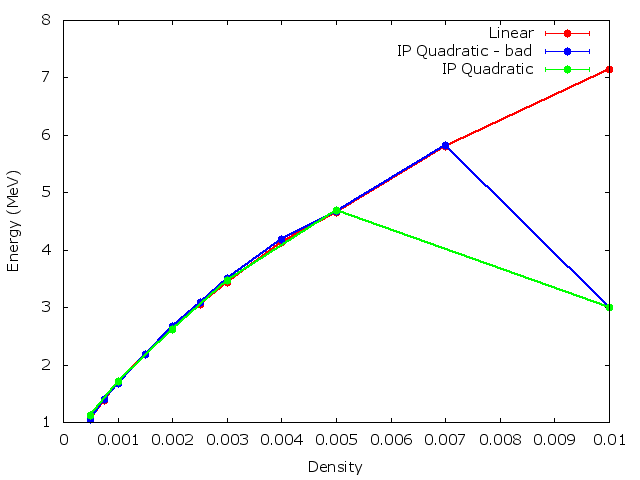
\includegraphics[width=\textwidth]{../14n_ke.png}
%      \caption{KE/particle for 14 neutrons.}
%   \end{subfigure}
%   ~
%   \begin{subfigure}{0.49\textwidth}
%      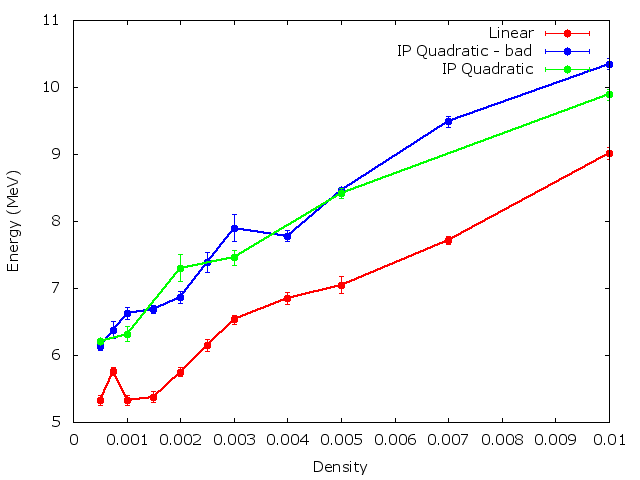
\includegraphics[width=\textwidth]{../14n2p_ke.png}
%      \caption{KE/particle for 14 neutrons + 2 protons.}
%   \end{subfigure}
%\end{figure}

%\section{Energy Plots for Alpha, 14n, and 14n2p - vc}
%\begin{figure}[h!]
%   \centering
%   \begin{subfigure}{0.49\textwidth}
%      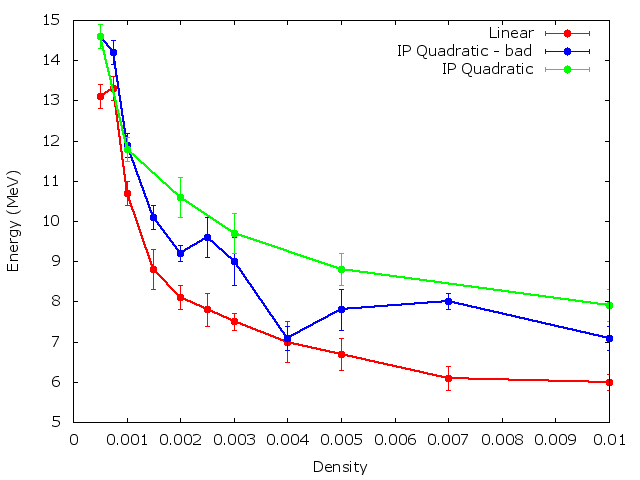
\includegraphics[width=\textwidth]{../alpha_vc.png}
%      \caption{vc of alpha calculated as $16\epsilon_{14n2p}-12\epsilon_{14n}$ where $\epsilon$ are the vc pieces of $\epsilon=E/A$.}
%   \end{subfigure}
%   ~
%   \begin{subfigure}{0.49\textwidth}
%      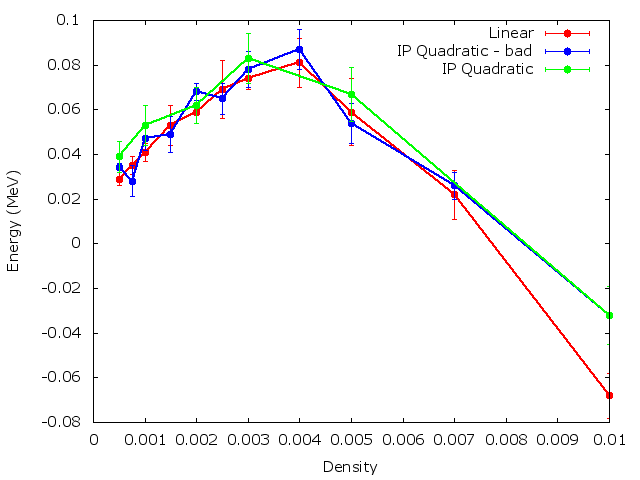
\includegraphics[width=\textwidth]{../14n_vc.png}
%      \caption{vc/particle for 14 neutrons.}
%   \end{subfigure}
%   ~
%   \begin{subfigure}{0.49\textwidth}
%      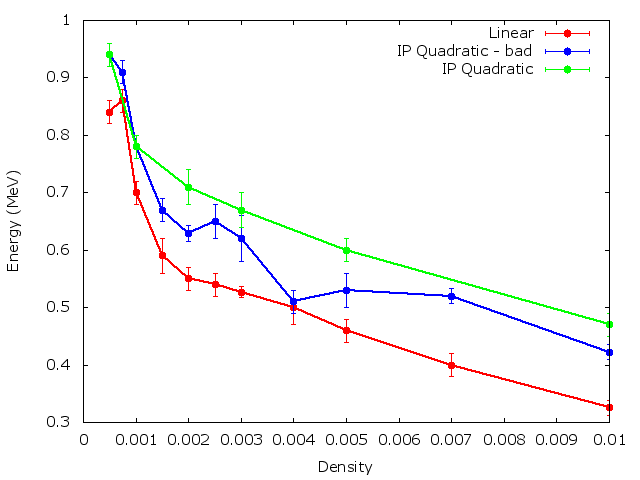
\includegraphics[width=\textwidth]{../14n2p_vc.png}
%      \caption{vc/particle for 14 neutrons + 2 protons.}
%   \end{subfigure}
%\end{figure}

\section{Breakdown of AV6' Potential Pieces with Linear Correlations}
\begin{figure}[h!]
   \centering
   \begin{subfigure}{0.49\textwidth}
      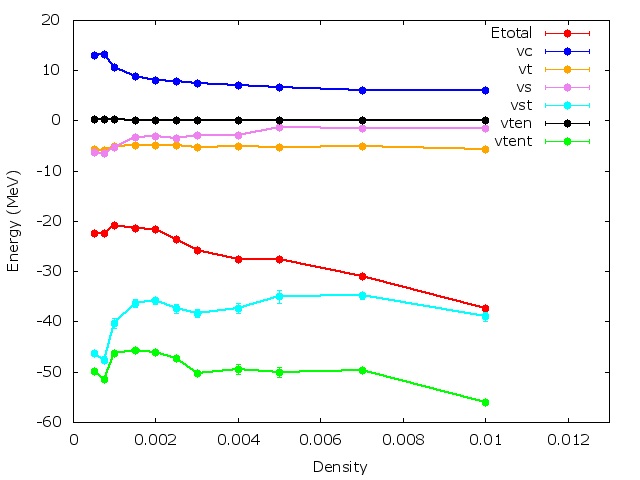
\includegraphics[width=\textwidth]{../av6_alpha_lin.png}
      \caption{Alpha energy calculated as $16\epsilon_{14n2p}-12\epsilon_{14n}$ where $\epsilon=E/A$.}
   \end{subfigure}
   ~
   \begin{subfigure}{0.49\textwidth}
      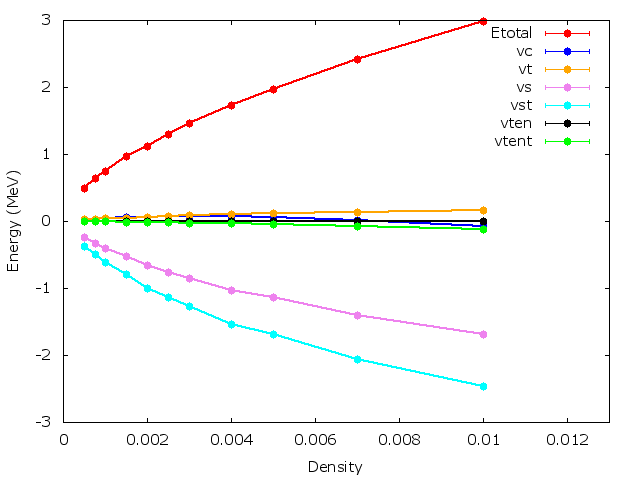
\includegraphics[width=\textwidth]{../av6_14n_lin.png}
      \caption{Energy/particle for 14 neutrons.}
   \end{subfigure}
   ~
   \begin{subfigure}{0.49\textwidth}
      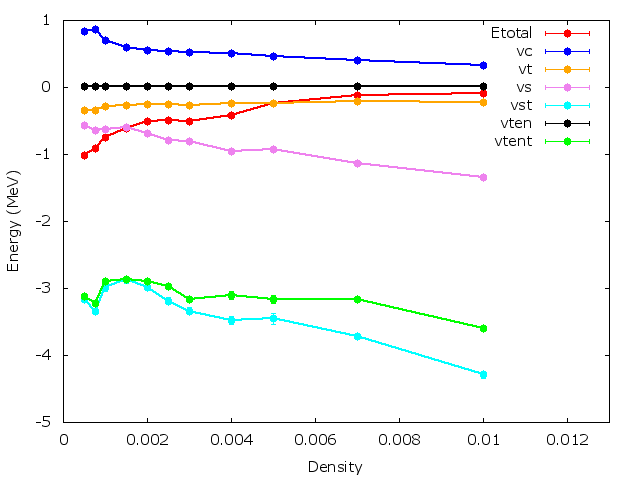
\includegraphics[width=\textwidth]{../av6_14n2p_lin.png}
      \caption{Energy/particle for 14 neutrons + 2 protons.}
   \end{subfigure}
\end{figure}
\newpage

\section{Breakdown of AV6' Potential Pieces with IP Correlations}
\begin{figure}[h!]
   \centering
   \begin{subfigure}{0.49\textwidth}
      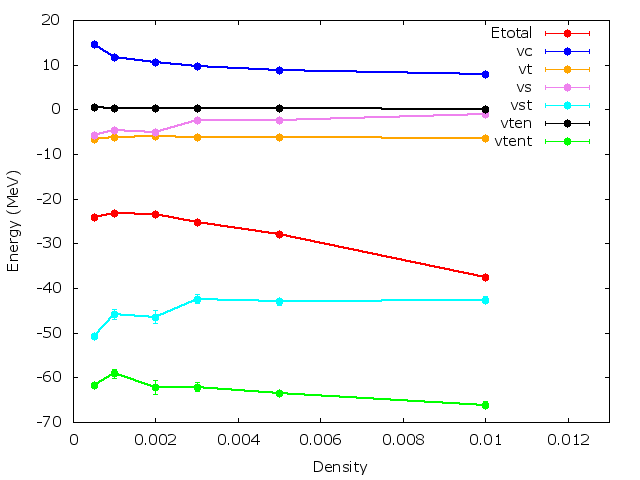
\includegraphics[width=\textwidth]{../av6_alpha_ip.png}
      \caption{Alpha energy calculated as $16\epsilon_{14n2p}-12\epsilon_{14n}$ where $\epsilon=E/A$.}
   \end{subfigure}
   ~
   \begin{subfigure}{0.49\textwidth}
      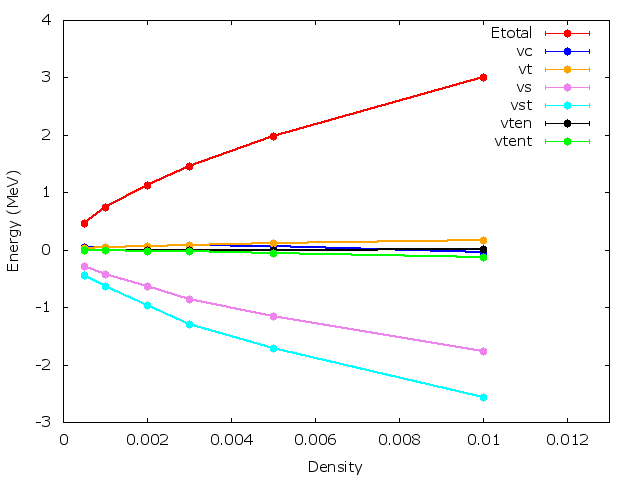
\includegraphics[width=\textwidth]{../av6_14n_ip.png}
      \caption{Energy/particle for 14 neutrons.}
   \end{subfigure}
   ~
   \begin{subfigure}{0.49\textwidth}
      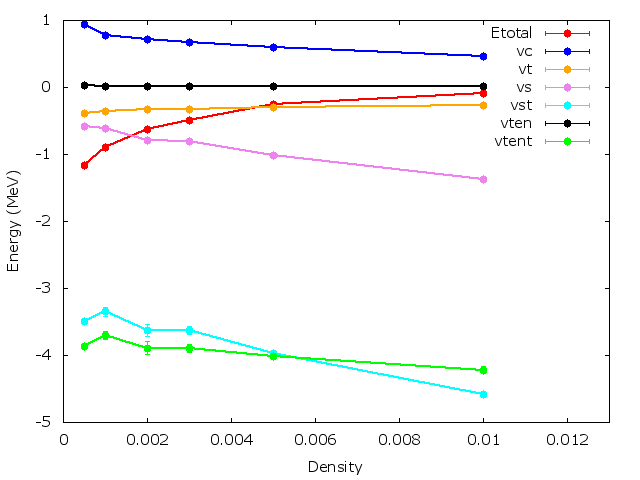
\includegraphics[width=\textwidth]{../av6_14n2p_ip.png}
      \caption{Energy/particle for 14 neutrons + 2 protons.}
   \end{subfigure}
\end{figure}
\newpage

\section{Breakdown of AV6' Potential Pieces with Both Linear and IP Correlations}
\begin{figure}[h!]
   \centering
   \begin{subfigure}{0.49\textwidth}
      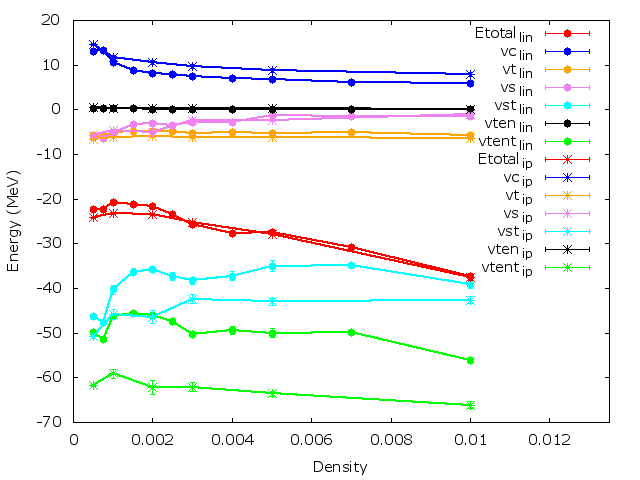
\includegraphics[width=\textwidth]{../av6_alpha_linVSip.png}
      \caption{Alpha energy calculated as $16\epsilon_{14n2p}-12\epsilon_{14n}$ where $\epsilon=E/A$.}
   \end{subfigure}
   ~
   \begin{subfigure}{0.49\textwidth}
      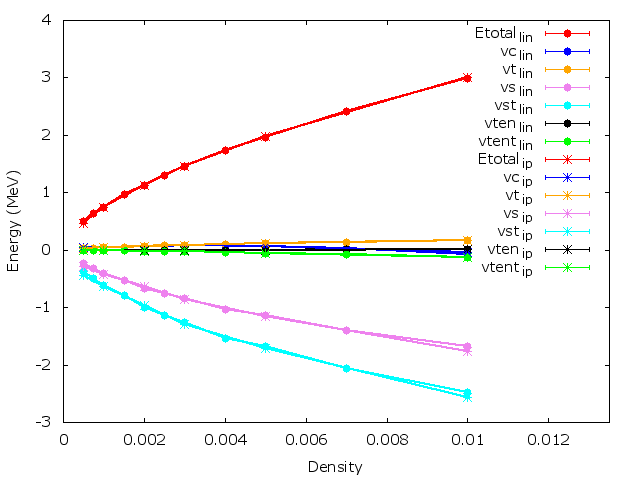
\includegraphics[width=\textwidth]{../av6_14n_linVSip.png}
      \caption{Energy/particle for 14 neutrons.}
   \end{subfigure}
   ~
   \begin{subfigure}{0.49\textwidth}
      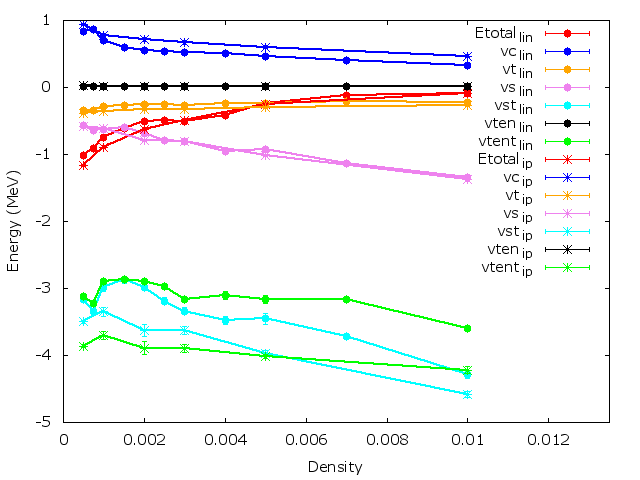
\includegraphics[width=\textwidth]{../av6_14n2p_linVSip.png}
      \caption{Energy/particle for 14 neutrons + 2 protons.}
   \end{subfigure}
\end{figure}
\newpage

\section{Distribution Functions for Linear and IP Correlations}
\begin{figure}[h!]
   \centering
   \begin{subfigure}{0.49\textwidth}
      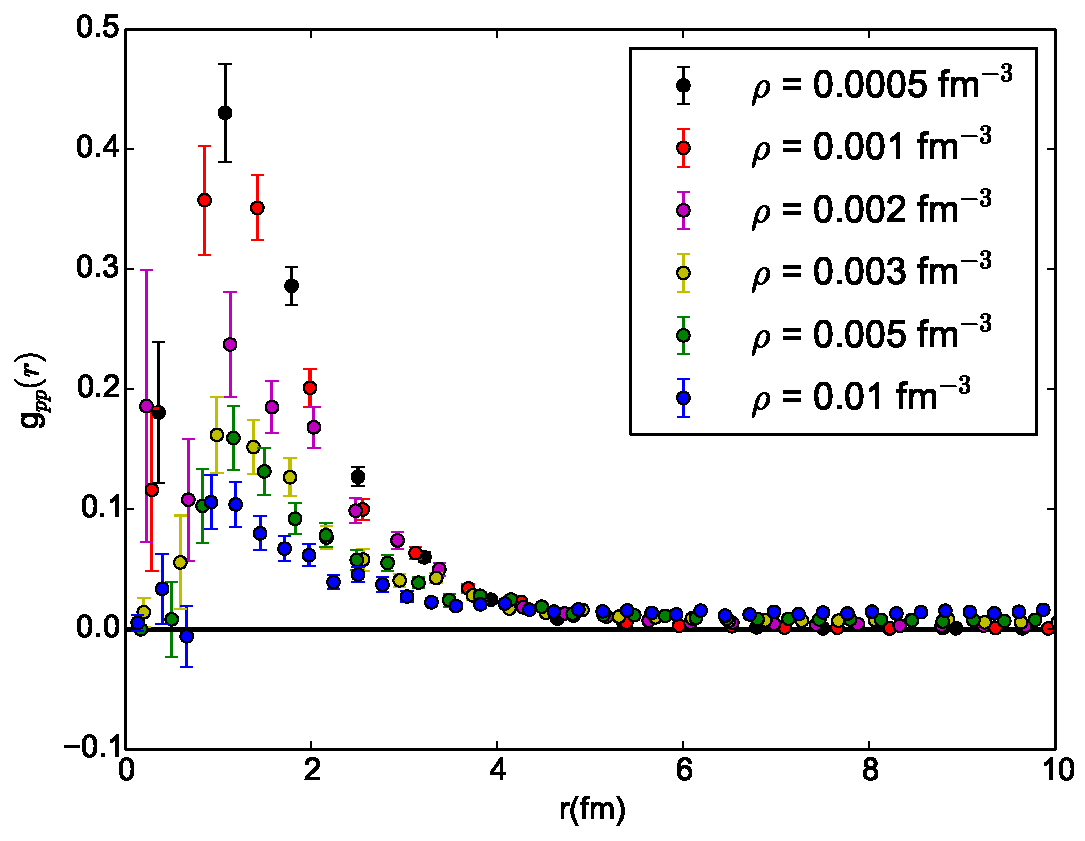
\includegraphics[width=\textwidth]{../gpp_lin.pdf}
      \caption{$g_{pp}(r)$ for linear correlations.}
   \end{subfigure}
   ~
   \begin{subfigure}{0.49\textwidth}
      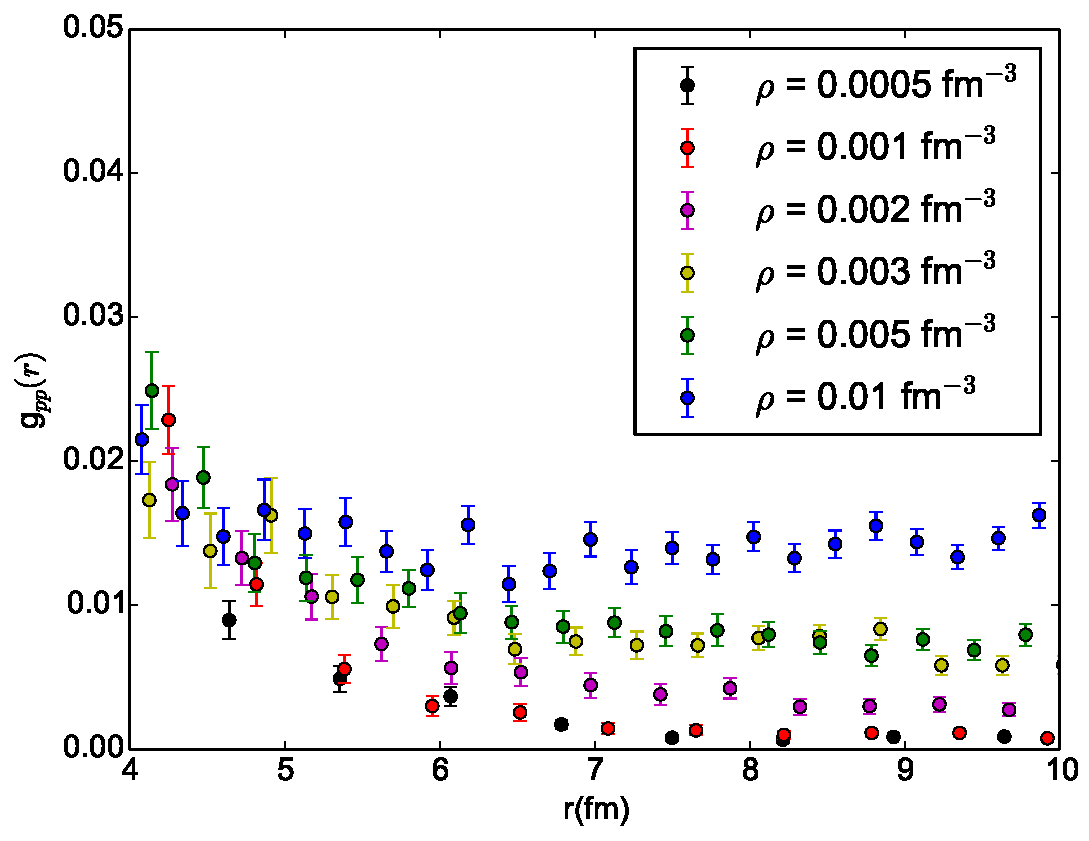
\includegraphics[width=\textwidth]{../gpp_lin_small.pdf}
      \caption{$g_{pp}(r)$ for linear correlations for high $r$.}
   \end{subfigure}
   ~
   \begin{subfigure}{0.49\textwidth}
      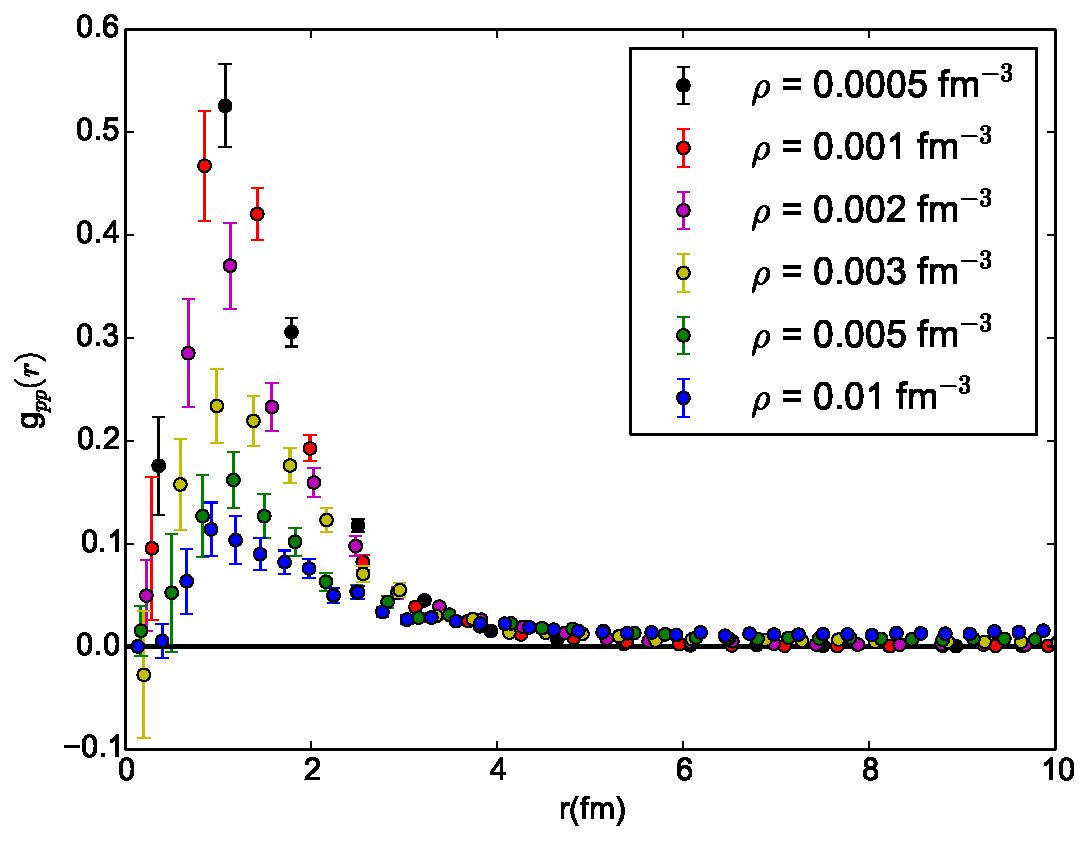
\includegraphics[width=\textwidth]{../gpp_ip.pdf}
      \caption{$g_{pp}(r)$ for IP correlations.}
   \end{subfigure}
   ~
   \begin{subfigure}{0.49\textwidth}
      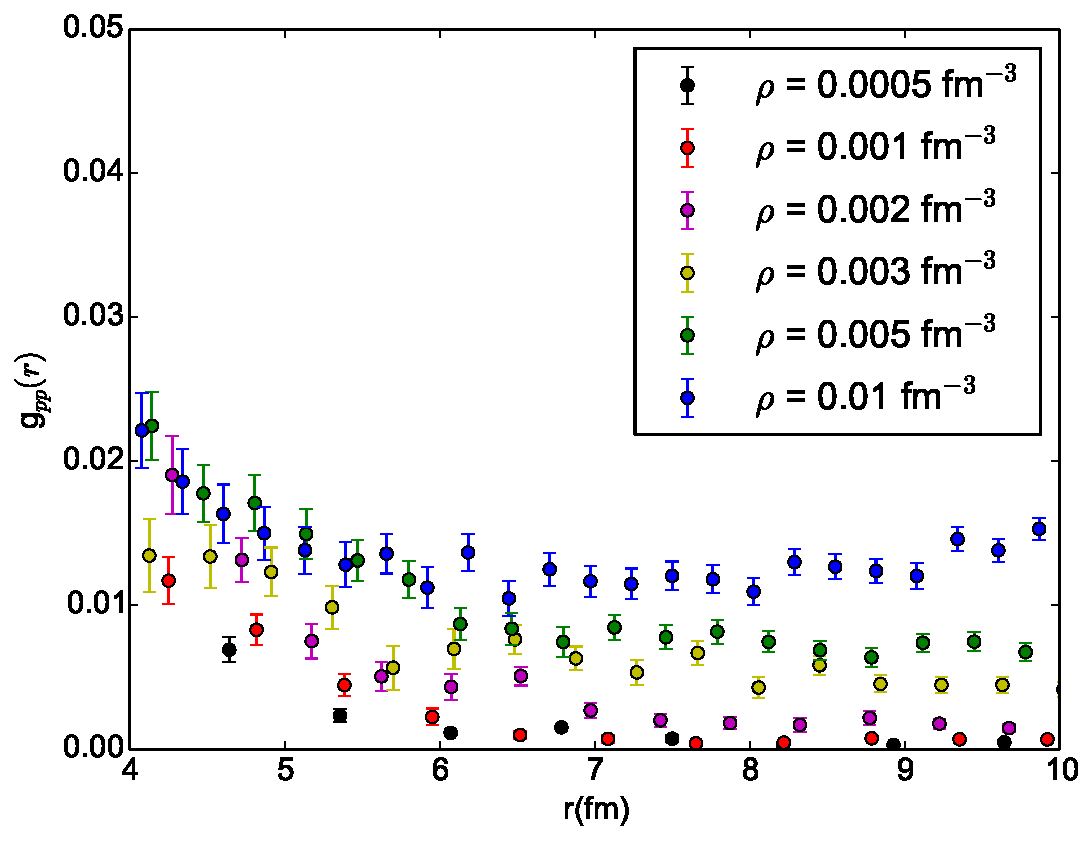
\includegraphics[width=\textwidth]{../gpp_ip_small.pdf}
      \caption{$g_{pp}(r)$ for IP correlations for high $r$.}
   \end{subfigure}
   ~
   \begin{subfigure}{0.49\textwidth}
      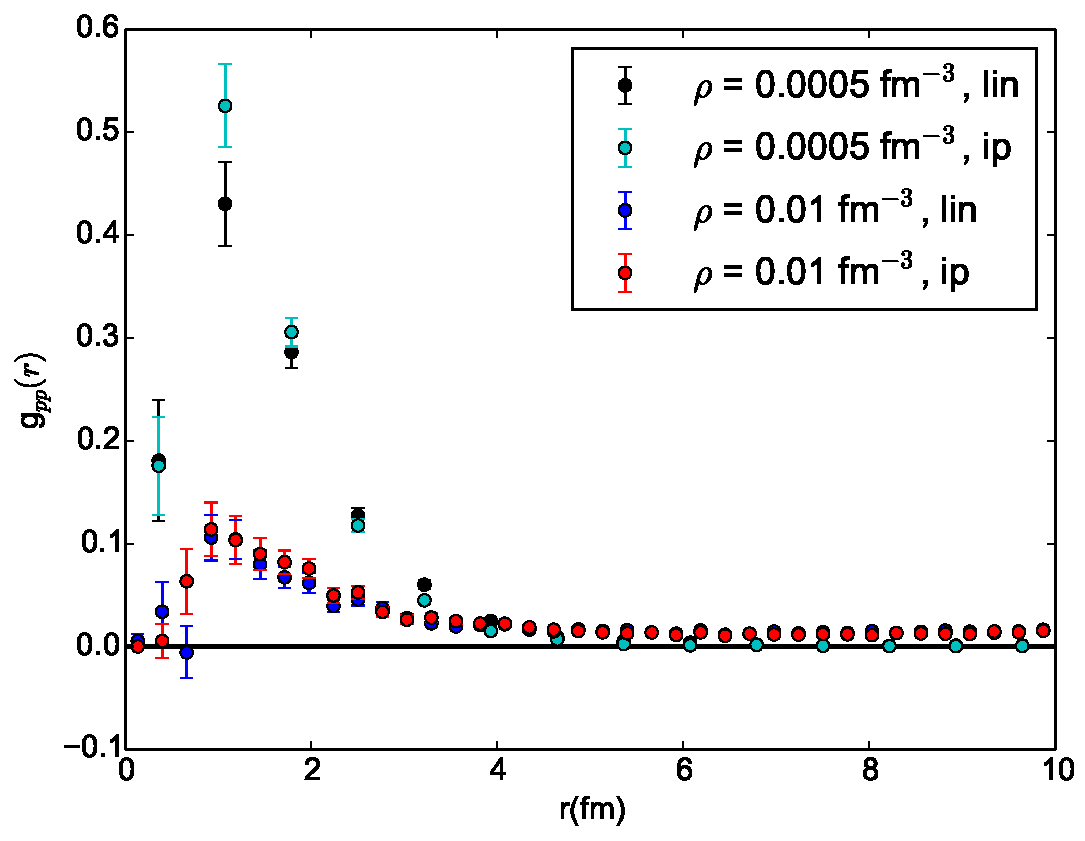
\includegraphics[width=\textwidth]{../gpp_linVSip.pdf}
      \caption{Comparison of $g_{pp}(r)$ for linear and IP correlations.}
   \end{subfigure}
   ~
   \begin{subfigure}{0.49\textwidth}
      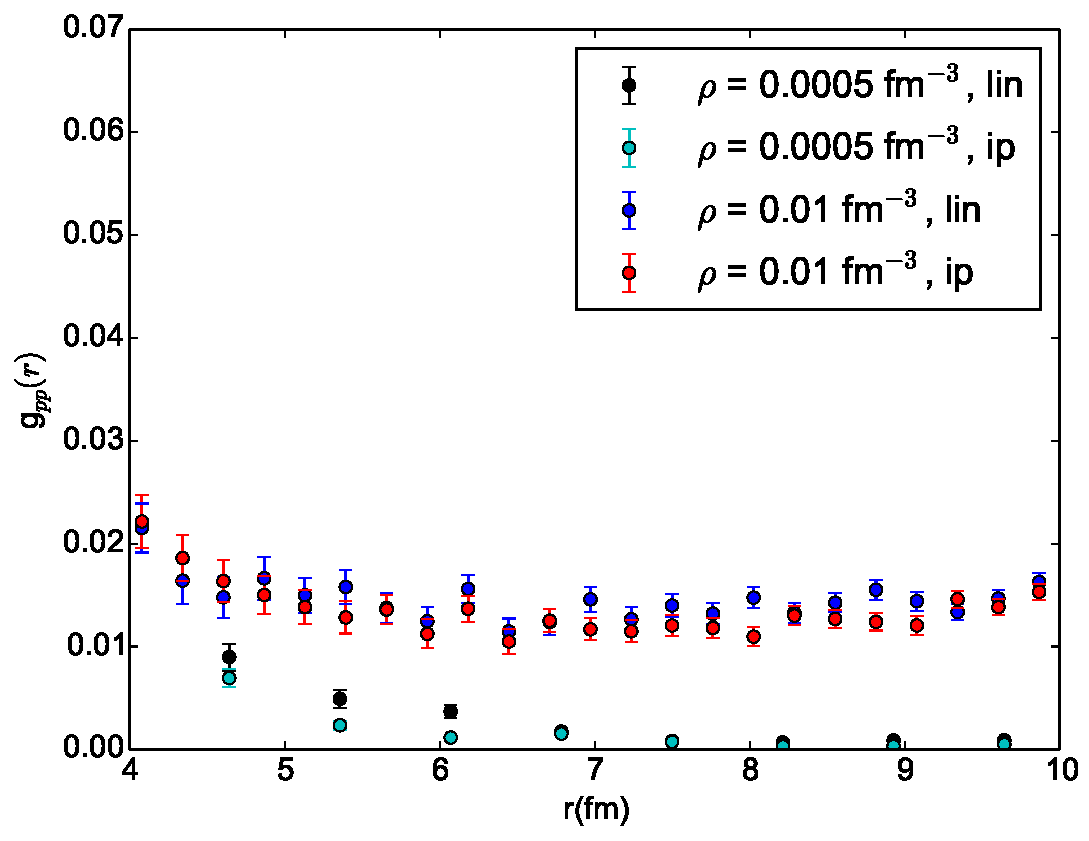
\includegraphics[width=\textwidth]{../gpp_linVSip_small.pdf}
      \caption{Comparison of $g_{pp}(r)$ for linear and IP correlations for high $r$.}
   \end{subfigure}
\end{figure}
Here we're looking at the $pp$ distribution function, like they used in \href{https://journals.aps.org/prl/pdf/10.1103/PhysRevLett.119.222505}{here} to look for alpha clusters.
\newpage



\clearpage
\bibliographystyle{unsrt}
\bibliography{../../papers/references}

\end{document}
